\documentclass[preprint,12pt,authoryear]{elsarticle}

%% Use the option review to obtain double line spacing
%% \documentclass[authoryear,preprint,review,12pt]{elsarticle}

\usepackage{amssymb}
\usepackage{amsmath}
\usepackage{graphicx}
\usepackage{hyperref}
\usepackage{lineno}

\journal{Computational Statistics \& Data Analysis}

\begin{document}

\begin{frontmatter}

\title{ORACLE: Online Anytime-Valid Causal Discovery}

\author[inst1]{Quang-Vinh Dang\corref{cor1}}
\ead{vinh.dq4@buv.edu.vn}
\cortext[cor1]{Corresponding author}

\affiliation[inst1]{organization={British University Vietnam},
            city={Hung Yen},
            country={Vietnam}}

\begin{abstract}
Causal discovery from streaming data is routinely performed by re-running a
batch estimator as new observations arrive and acting on the first graph that
``looks significant.'' This data-dependent, repeated-looks usage voids the
fixed-sample error guarantees of the underlying tests: the probability of
declaring a spurious edge grows without bound as the stream lengthens. We
present ORACLE, an online causal discovery procedure that controls the false
edge rate \emph{at every stopping time} with no correction for the number of
looks. ORACLE replaces the conditional-independence $p$-value at the heart of
constraint-based discovery with a sequential test by betting: each candidate
relationship is monitored by a nonnegative martingale (betting wealth) built
from a kernelized witness, so that a rejection the first time the wealth exceeds
$1/\alpha$ is anytime-valid by Ville's inequality. Conditional independence is
reduced to unconditional independence by previsible online residualisation;
edges are oriented by the additive-noise asymmetry, rejecting the anti-causal
direction whose residual remains dependent on its input; per-edge wealths are
combined by e-BH for false discovery rate control; and mechanism shifts are
flagged by a Page--CUSUM on the edgewise log-wealth increments. On synthetic
additive-noise structural causal models we show that ORACLE keeps the
family-wise error below the nominal level uniformly over the stream while a
naive optional-stopping baseline inflates to nearly one, that it recovers graph
structure competitively with batch constraint- and score-based methods, and
that its change detector traces a controllable delay/false-alarm trade-off, all
at streaming throughput.
\end{abstract}

\begin{keyword}
causal discovery \sep anytime-valid inference \sep e-values \sep sequential testing \sep change-point detection
\end{keyword}

\end{frontmatter}

%% Optional: To add line numbers (often requested during review)
% \linenumbers

%% ===================================================================
\section{Introduction}
\label{sec:intro}
Many systems that demand causal understanding---financial markets, intensive-care
monitoring, industrial process lines, sensor networks---produce data as an
unbounded stream rather than a fixed sample. A practitioner who wants an
up-to-date causal graph from such a stream typically re-runs a batch discovery
algorithm at regular intervals and reacts to the structure as soon as it appears
stable or significant. This is statistically unsound. Classical discovery
algorithms control error only at a single, pre-specified sample size; querying
them repeatedly and stopping at a data-dependent time is a form of optional
stopping that inflates the type-I error. With $T$ looks at a level-$\alpha$
$p$-value test, the chance of at least one false rejection approaches one as
$T$ grows, and no fixed multiplicity correction repairs this because the number
of looks is itself unbounded and data-dependent.

We address this with ORACLE, an \emph{online, anytime-valid} causal discovery
procedure. The guiding principle is to attach to every candidate causal claim a
test statistic that is valid not merely at one sample size but simultaneously at
\emph{all} sample sizes, so that an analyst may inspect the running estimate as
often as desired and stop whenever convenient without spending any error budget
on the looking. The technical vehicle is testing by betting: each candidate
relationship is monitored by a nonnegative martingale---a betting wealth
process---that, under the null hypothesis of no edge, never grows in
expectation. Ville's inequality then bounds the probability that the wealth ever
crosses $1/\alpha$ by $\alpha$, making the rejection rule ``declare an edge the
first time the wealth reaches $1/\alpha$'' anytime-valid by construction.

Building a full causal-discovery pipeline on this foundation requires more than a
single test. We must (i) construct a \emph{valid} sequential independence test
whose increments are genuine e-values, (ii) extend it to conditional
independence so that the recovered object is a directed acyclic graph (DAG)
rather than a marginal dependency graph, (iii) orient edges with the correct
additive-noise asymmetry, (iv) combine evidence across the quadratically many
candidate edges with multiplicity control that also respects optional stopping,
and (v) detect when the underlying mechanism changes. ORACLE supplies each
component while preserving previsibility---every tuning quantity (bandwidths,
bet sizes, regression fits) is a function of strictly past data---so that the
anytime guarantee is never silently broken.

\paragraph{Contributions.}
(1) A valid sequential kernelized independence test whose betting wealth is a
nonnegative martingale under the null, obtained from an exchangeability-based
swap construction with a previsible, scale-standardised witness
(Section~\ref{sec:method}). (2) A streaming conditional-independence test by
previsible online residualisation, yielding consistent skeleton recovery when
conditioning on the estimated parent set. (3) An online additive-noise
orientation rule that orients edges by rejecting the anti-causal direction,
together with e-BH multiplicity control and an incremental DAG projection.
(4) A Page--CUSUM change detector on edgewise log-wealth increments that
monitors mechanism validity. (5) An empirical study showing uniform-in-time
error control, competitive structure recovery, a controllable detection
delay/false-alarm trade-off, and streaming throughput, including a falsification
experiment that exhibits the optional-stopping inflation ORACLE is designed to
avoid (Section~\ref{sec:results}).

%% ===================================================================
\section{Related Work}
\label{sec:related}

\paragraph{Causal discovery: classical and continuous-optimization foundations.}
Causal structure learning has classically been approached through constraint-based and score-based search over the space of directed acyclic graphs \cite{spirtes2000causation, pearl2009causality, peters2017elements}, with order-independent constraint-based learning \cite{colombo2014pcstable} and greedy score-based identification \cite{chickering2002ges} serving as canonical references. A subsequent line of work recast structure learning as continuous optimization with a smooth acyclicity constraint \cite{zheng2018notears}, extended to nonparametric mechanisms \cite{zheng2020sparsedag}, graph neural networks \cite{yu2019daggnn}, interventional data \cite{brouillard2020dcdi}, and fully Bayesian posteriors over graphs \cite{lorch2021dibs}. Identifiability in the purely observational setting is most cleanly characterized for additive noise models \cite{hoyer2008anm, peters2014canm}, in which the true direction is the one yielding residuals independent of the inputs. Our method builds directly on this independence-of-residuals principle, and we adopt the structural intervention distance \cite{peters2015sid} as a causally meaningful evaluation metric alongside structural Hamming distance.

\paragraph{Independence testing and kernel dependence measures.}
Detecting (conditional) dependence is the statistical core of constraint-based discovery. The Hilbert--Schmidt Independence Criterion \cite{gretton2005hsic} and the associated kernel two-sample test \cite{gretton2012mmd} provide nonparametric dependence measures that underpin many discovery pipelines. These are batch tests: they fix the sample size in advance and lose validity under repeated inspection of a growing stream. Our work instead requires a test that remains valid under continuous monitoring.

\paragraph{E-values, test martingales, and safe anytime-valid inference.}
The framework of game-theoretic statistics and safe anytime-valid inference \cite{ramdas2023savi} provides exactly this guarantee: by replacing $p$-values with e-values and accumulating evidence multiplicatively into a test martingale \cite{grunwald2024safetesting, ramdas2025evalues}, type-I error is controlled uniformly over all stopping times via Ville's inequality \cite{ville1939}. E-values further support powerful multiplicity control through the e-BH procedure \cite{wang2022ebh}, which we use for family-wise edge control. The principle of testing by betting has produced sequential kernelized independence tests \cite{podkopaev2023skit}, sequential conditional independence tests \cite{shaer2023modelx}, and nonparametric two-sample tests \cite{shekhar2023twosample}; ORACLE adopts the sequential kernelized betting construction as its per-edge evidence process, in place of the invalid fixed-sample statistic used in prior streaming heuristics.

\paragraph{Online, nonstationary, and time-series causal discovery.}
Several methods relax the stationarity and batch assumptions. CD-NOD recovers causal structure from heterogeneous and nonstationary data via a surrogate domain index \cite{huang2020cdnod}, and has been extended to lagged time-series settings \cite{sadeghi2025cdnots}. Other recent approaches handle non-stationarity through minimum-description-length scoring with regime change-points \cite{mameche2025spacetime}, conditional stationarity given latent states \cite{balsellsrodas2025sdci}, and contemporaneous-plus-lagged conditional independence search \cite{runge2020pcmciplus}. Unlike these methods, all of which provide either asymptotic guarantees or none, ORACLE provides finite-sample error control at every stopping time.

\paragraph{Change-point and shift detection in causal models.}
Detecting when a causal mechanism changes connects our shift-detection module to the classical change-point literature: cumulative-sum schemes \cite{page1954cusum} with optimal-delay analysis \cite{lorden1971} form the basis of our wealth-process monitor. Recent work studies change-point detection and localization specifically for causal models \cite{huang2024ccp}, discovery-driven change-point detection in time series \cite{gao2025cdcpd}, and quickest causal change-point detection under adaptive intervention \cite{xu2025quickestccp}. ORACLE reuses its existing martingale wealth process for shift detection, incurring no additional per-edge testing overhead.

\paragraph{Amortized and foundation-model causal discovery.}
A rapidly growing direction trains models on simulated structural causal models and amortizes inference to a single forward pass \cite{lorch2022avici, ke2023csiva, wu2024sea}, with recent in-context and prior-data-fitted variants \cite{balazadeh2025causalpfn, robertson2025dopfn, swelam2025tabpfn}. While fast and competitive on in-distribution synthetic data, these models are inherently batch, offer no per-instance error guarantee, and remain bound by identifiability limits \cite{montagna2025demystifying}. Concurrent 2026 work continues to push amortized and search-based discovery for nonstationary time series \cite{castillo2026tsboss, faruque2026ttcd}, underscoring the timeliness of streaming causal discovery while leaving the anytime-validity gap open.

\paragraph{Benchmarks and evaluation.}
Reliable evaluation requires care: simulated DAG benchmarks can be trivially gamed through marginal-variance artifacts \cite{reisach2021beware}, motivating normalization of synthetic data. We therefore additionally evaluate on realistic and ground-truthed benchmarks, including realistically generated time series \cite{cheng2024causaltime}, production-process data \cite{gobler2024causalassembly}, large-scale real-world river networks \cite{stein2025causalrivers}, and dynamical-system benchmarks \cite{herdeanu2025causaldynamics}.

%% ===================================================================
\section{Problem Setting and Preliminaries}
\label{sec:prelim}
\paragraph{Streaming structural causal model.}
Observations $X_1, X_2, \dots \in \mathbb{R}^p$ arrive sequentially from a
(piecewise-)stationary structural causal model (SCM). At each time $t$ the
procedure outputs an estimated DAG $\hat G_t$ over the $p$ variables and,
optionally, change alarms. We work under the standard identifiability
assumptions: (A1) causal sufficiency (no unobserved confounders); (A2)
faithfulness; (A3) an additive non-Gaussian noise mechanism
\begin{equation}
    X_j = f_j\!\left(X_{\mathrm{Pa}(j)}\right) + \varepsilon_j,
    \qquad \varepsilon_j \perp\!\!\!\perp X_{\mathrm{Pa}(j)},
    \label{eq:anm}
\end{equation}
with the noise non-Gaussian or the mechanism nonlinear so that the direction is
identified; and (A4) a characteristic kernel for the independence tests. Under
(A1)--(A4) the graph is identifiable from the joint distribution, and the task
is to recover it online while controlling error under optional stopping.

\paragraph{e-values, e-processes and anytime validity.}
An \emph{e-variable} for a null $H_0$ is a nonnegative random variable $E$ with
$\mathbb{E}_{H_0}[E] \le 1$. An \emph{e-process} is a sequence $(E_t)_{t\ge 1}$
that is upper-bounded by a nonnegative supermartingale under every
$P \in H_0$. Ville's inequality states that for a nonnegative supermartingale
$(K_t)$ with $K_0 = 1$,
\begin{equation}
    P\!\left(\, \exists\, t : K_t \ge 1/\alpha \,\right) \le \alpha .
    \label{eq:ville}
\end{equation}
Hence the rule ``reject $H_0$ the first time $K_t \ge 1/\alpha$'' has type-I
error at most $\alpha$ \emph{simultaneously over all $t$}, i.e. at any
data-dependent stopping time, with no penalty for the number of looks. This is
precisely the property a streaming discovery method needs.

\paragraph{Testing by betting.}
A constructive route to such a $K_t$ is to play a fictitious game: starting with
unit wealth, at each round we place a previsible bet $\lambda_t \in [0,1)$ on a
payoff $g_t$ with $\mathbb{E}_{H_0}[g_t \mid \mathcal{F}_{t-1}] \le 0$ and
$|g_t| \le 1$, updating
\begin{equation}
    K_t = K_{t-1}\,(1 + \lambda_t\, g_t).
    \label{eq:wealth}
\end{equation}
Then $(K_t)$ is a nonnegative martingale (supermartingale) under $H_0$, so
\eqref{eq:ville} applies, while under the alternative a well-chosen bet makes
the wealth grow, giving power. The entire design problem is to construct, for
each causal hypothesis, a payoff $g_t$ that is (i) a valid e-value increment
under the null and (ii) informative under the alternative---using only past data
to remain previsible.

%% ===================================================================
\section{Methodology}
\label{sec:method}
ORACLE maintains, per ordered pair and node, an estimated parent set, online
regressors, skeleton and orientation betting wealths, and a change-detection
statistic. We describe each component, then the per-timestep pipeline and the
guarantees.

\subsection{A valid sequential independence test (SKIT)}
\label{sec:skit}
We test $H_0\!: U \perp\!\!\!\perp V$ from a stream of paired samples
$(u_t, v_t)$. The key to validity is an \emph{exchangeability} construction.
Processing two fresh pairs $(u_a,v_a)$, $(u_b,v_b)$ at a time, define the
\emph{joint} points $P=\{(u_a,v_a),(u_b,v_b)\}$ and the \emph{product} (swapped)
points $Q=\{(u_a,v_b),(u_b,v_a)\}$. Under $H_0$ the joint law equals the product
law, so the multiset $\{P,Q\}$ is exchangeable: relabelling joint $\leftrightarrow$
product does not change its distribution. With any previsible witness function
$f_t$ (built from data strictly before the current round) we set the payoff
\begin{equation}
    g_t = \tfrac{1}{2}\Big(\textstyle\frac{1}{2}\!\sum_{x\in P} f_t(x)
          - \frac{1}{2}\!\sum_{x\in Q} f_t(x)\Big),
    \qquad f_t \in [-1,1].
    \label{eq:payoff}
\end{equation}
Exchangeability gives $\mathbb{E}_{H_0}[g_t \mid \mathcal{F}_{t-1}] = 0$ for
\emph{any} previsible $f_t$, and clipping $f_t$ to $[-1,1]$ ensures
$|g_t|\le 1$, so $1+\lambda_t g_t > 0$ and the wealth \eqref{eq:wealth} stays
nonnegative. Crucially, validity does not depend on the quality of the
witness---only power does.

For the witness we use the kernel mean-embedding difference between the joint
and product measures (the HSIC witness), estimated online with Random Fourier
Features (RFF) so that the per-round cost is $O(D^2)$ with $O(D^2)$ memory and no
growing sample. Because the raw HSIC signal is small in magnitude, we
\emph{standardise} the witness by its running scale (the root-mean-square of past
witness evaluations), turning a weak signal into an order-one payoff; the scale
is previsible, so the null mean-zero property of \eqref{eq:payoff} is preserved.
Bet sizing $\lambda_t$ defaults to a parameter-free mixture-of-bets (a grid of
fixed bets whose wealths are averaged), with previsible aGRAPA and fixed-$\lambda$
variants available. Bandwidths are fixed from a warm-up window and never
recomputed on the current point, preserving previsibility.

\subsection{Conditional independence by residual reduction}
\label{sec:ci}
To recover a DAG rather than a dependency graph we must condition. We adopt the
RESIT-style reduction: maintain previsible online regressors
$\hat f_{U\mid S}$ and $\hat f_{V\mid S}$ (RFF ridge by recursive least squares),
residualise $\tilde u_t = u_t - \hat f_{U\mid S}(s_t)$ and
$\tilde v_t = v_t - \hat f_{V\mid S}(s_t)$, and run the SKIT test of
Section~\ref{sec:skit} on the residual stream. Under the additive structure
\eqref{eq:anm}, $U \perp\!\!\!\perp V \mid S$ is equivalent to independence of the
residuals, and predicting-then-updating keeps the residuals previsible. With an
empty conditioning set this reduces exactly to the unconditional test.

\subsection{Orientation by additive-noise asymmetry}
\label{sec:orient}
For an adjacent pair $\{i,j\}$ we exploit the ANM asymmetry. Let
$a_t = X_{j,t} - \hat f_{j\mid i}(X_{i,t})$ be the forward residual ($i\to j$)
and $b_t = X_{i,t} - \hat f_{i\mid j}(X_{j,t})$ the reverse residual ($j\to i$).
We run two SKIT wealths, $A$ testing dependence of $a$ on $X_i$ and $B$ testing
dependence of $b$ on $X_j$. The correct rule \emph{rejects the anti-causal
direction}: a true edge $i\to j$ implies $a \perp\!\!\!\perp X_i$ (so $A$ stays
low) and $b \not\!\perp\!\!\!\perp X_j$ (so $B$ grows). Hence
\begin{equation}
\hat e_{ij} =
\begin{cases}
 i \to j, & B \ge 1/\alpha \text{ and } A < 1/\alpha,\\
 j \to i, & A \ge 1/\alpha \text{ and } B < 1/\alpha,\\
 \text{undirected}, & \text{otherwise.}
\end{cases}
\label{eq:orient}
\end{equation}
When both wealths grow---a signature of misspecification or hidden
confounding---ORACLE leaves the edge undirected rather than guessing, surfacing
its own failure mode. The sign convention is the crux of the method and is
unit-tested on a two-node graph with known ground truth.

\subsection{Multiplicity, DAG projection, and change detection}
\label{sec:multdag}
\paragraph{e-BH false discovery control.}
Each surviving edge contributes its rejecting wealth as a valid e-value. Across
the $K = p(p-1)/2$ candidate edges we apply e-BH \citep{wang2022ebh}: sort the
e-values $e_{(1)} \ge \dots \ge e_{(K)}$ and reject the top $k^\star$ where
$k^\star = \max\{k : e_{(k)} \ge K/(\alpha k)\}$. e-BH controls the FDR for
arbitrarily dependent e-values---exactly our regime, since edge wealths share
the stream---and an e-Bonferroni threshold $K/\alpha$ is available as the
conservative family-wise option.

\paragraph{Incremental DAG projection.}
Oriented, surviving edges are added in decreasing order of log-wealth margin; an
edge that would close a cycle is dropped, so the lowest-confidence edge in any
cycle is removed. We report both the pre- and post-projection graphs.

\paragraph{Page--CUSUM change detection.}
For each active edge we monitor mechanism validity with a residual monitor whose
wealth is flat while the fitted model is correct (residual independent of input)
and rises when the mechanism changes. A Page--CUSUM on its log e-increments,
\begin{equation}
    G_t = \max\!\left(0,\; G_{t-1} + \log e_t - c\right),
    \label{eq:cusum}
\end{equation}
alarms when $G_t > h$; the threshold $h$ trades detection delay against the
average run length (ARL) to false alarm, and an alarm resets the affected
wealths to $K=1$ so that post-change evidence accumulates cleanly.

\subsection{Guarantees and complexity}
\label{sec:guarantees}
By construction each per-edge wealth is a nonnegative martingale under its null,
so by \eqref{eq:ville} the per-edge type-I error is at most $\alpha$ at every
stopping time; e-BH lifts this to anytime FDR control and e-Bonferroni to
anytime FWER control. Under (A1)--(A4), conditioning on the estimated parent set
makes the skeleton test consistent, so $\hat G_t \to G^\star$ almost surely. The
Page--CUSUM inherits the standard delay scaling $O(h / \mathrm{KL})$ against a
controllable ARL. Per timestep, the residual regressors and wealth updates cost
$O(p^2 D^2)$ with the degree cap $k$ controlling the conditioning cost; we use
$k \le 2$, Markov-blanket pruning of conditioning sets, and $D \approx 64$ RFF
features to keep the method real-time for moderate $p$. We emphasise that the
error guarantee assumes each per-edge increment is a valid e-value---a
mild, construction-level assumption---and not ``no assumptions on the
data-generating process.''

%% ===================================================================
\section{Experimental Setup}
\label{sec:setup}
\paragraph{Data.}
Our primary workhorse is synthetic additive-noise SCMs on random DAGs
(Erd\H{o}s--R\'enyi and scale-free, $p \in \{5,\dots,50\}$, varying density)
with non-Gaussian noise (Laplace, Student-$t_3$) and nonlinear mechanisms. We
generate the data ourselves so the ground-truth graph and any planted
change-points are known exactly. Following the cautionary findings on simulated
DAGs, we standardise every variable and verify low \emph{varsortability}, which
falls from $\approx 0.96$ on raw data to $\approx 0.39$ after normalisation; all
graph-recovery results are reported on normalised data so that marginal-variance
ordering cannot leak the topological order. For change detection we generate
piecewise-stationary streams with planted change-points at which mechanisms
change, and for the validity audit we generate null streams of $p$ mutually
independent series (no edges).

\paragraph{Baselines.}
The central comparator is a \emph{naive optional-stopping} procedure: a standard
permutation HSIC test recomputed on the growing sample at every look, declaring
an edge the first time $p<\alpha$ with no multiplicity or repeated-looks
correction---the precise failure mode ORACLE is designed to avoid. We also
compare against batch constraint- and score-based discovery (PC-stable with
Fisher-Z and KCI tests, and GES with the BIC score) run in a checkpoint harness,
and a kernel change-point detector for the change experiments.

\paragraph{Metrics.}
For ground-truthed data we report structural Hamming distance (SHD), structural
intervention distance (SID), and precision/recall/F1 separately for skeleton
adjacency and edge orientation. For the anytime claim we report empirical
family-wise and per-edge type-I error as a function of stream length, evaluated
at all $t$ simultaneously with the $\alpha$ line overlaid. For change detection
we report the detection delay against the ARL to false alarm. For systems we
report throughput (observations/second) and peak memory versus $p$.

%% ===================================================================
\section{Results}
\label{sec:results}
\paragraph{Validity audit: the falsification test.}
On a null stream of mutually independent series
(Figure~\ref{fig:validity}), ORACLE's SKIT wealth keeps the maximum per-edge
type-I error at $0.04$ and the e-Bonferroni family-wise error at $0.01$, both at
or below the nominal $\alpha = 0.05$ \emph{uniformly over the stream}. The naive
optional-stopping baseline, by contrast, inflates to a per-edge error of $0.47$
and a family-wise error of $0.98$, climbing monotonically with stream length.
This is the single most important experiment: it confirms that the corrected
betting construction controls error under optional stopping, whereas the usual
repeated-looks usage of a fixed-sample test does not, and a design whose
increments are not valid e-values would diverge here immediately.

\begin{figure}[htpb]
    \centering
    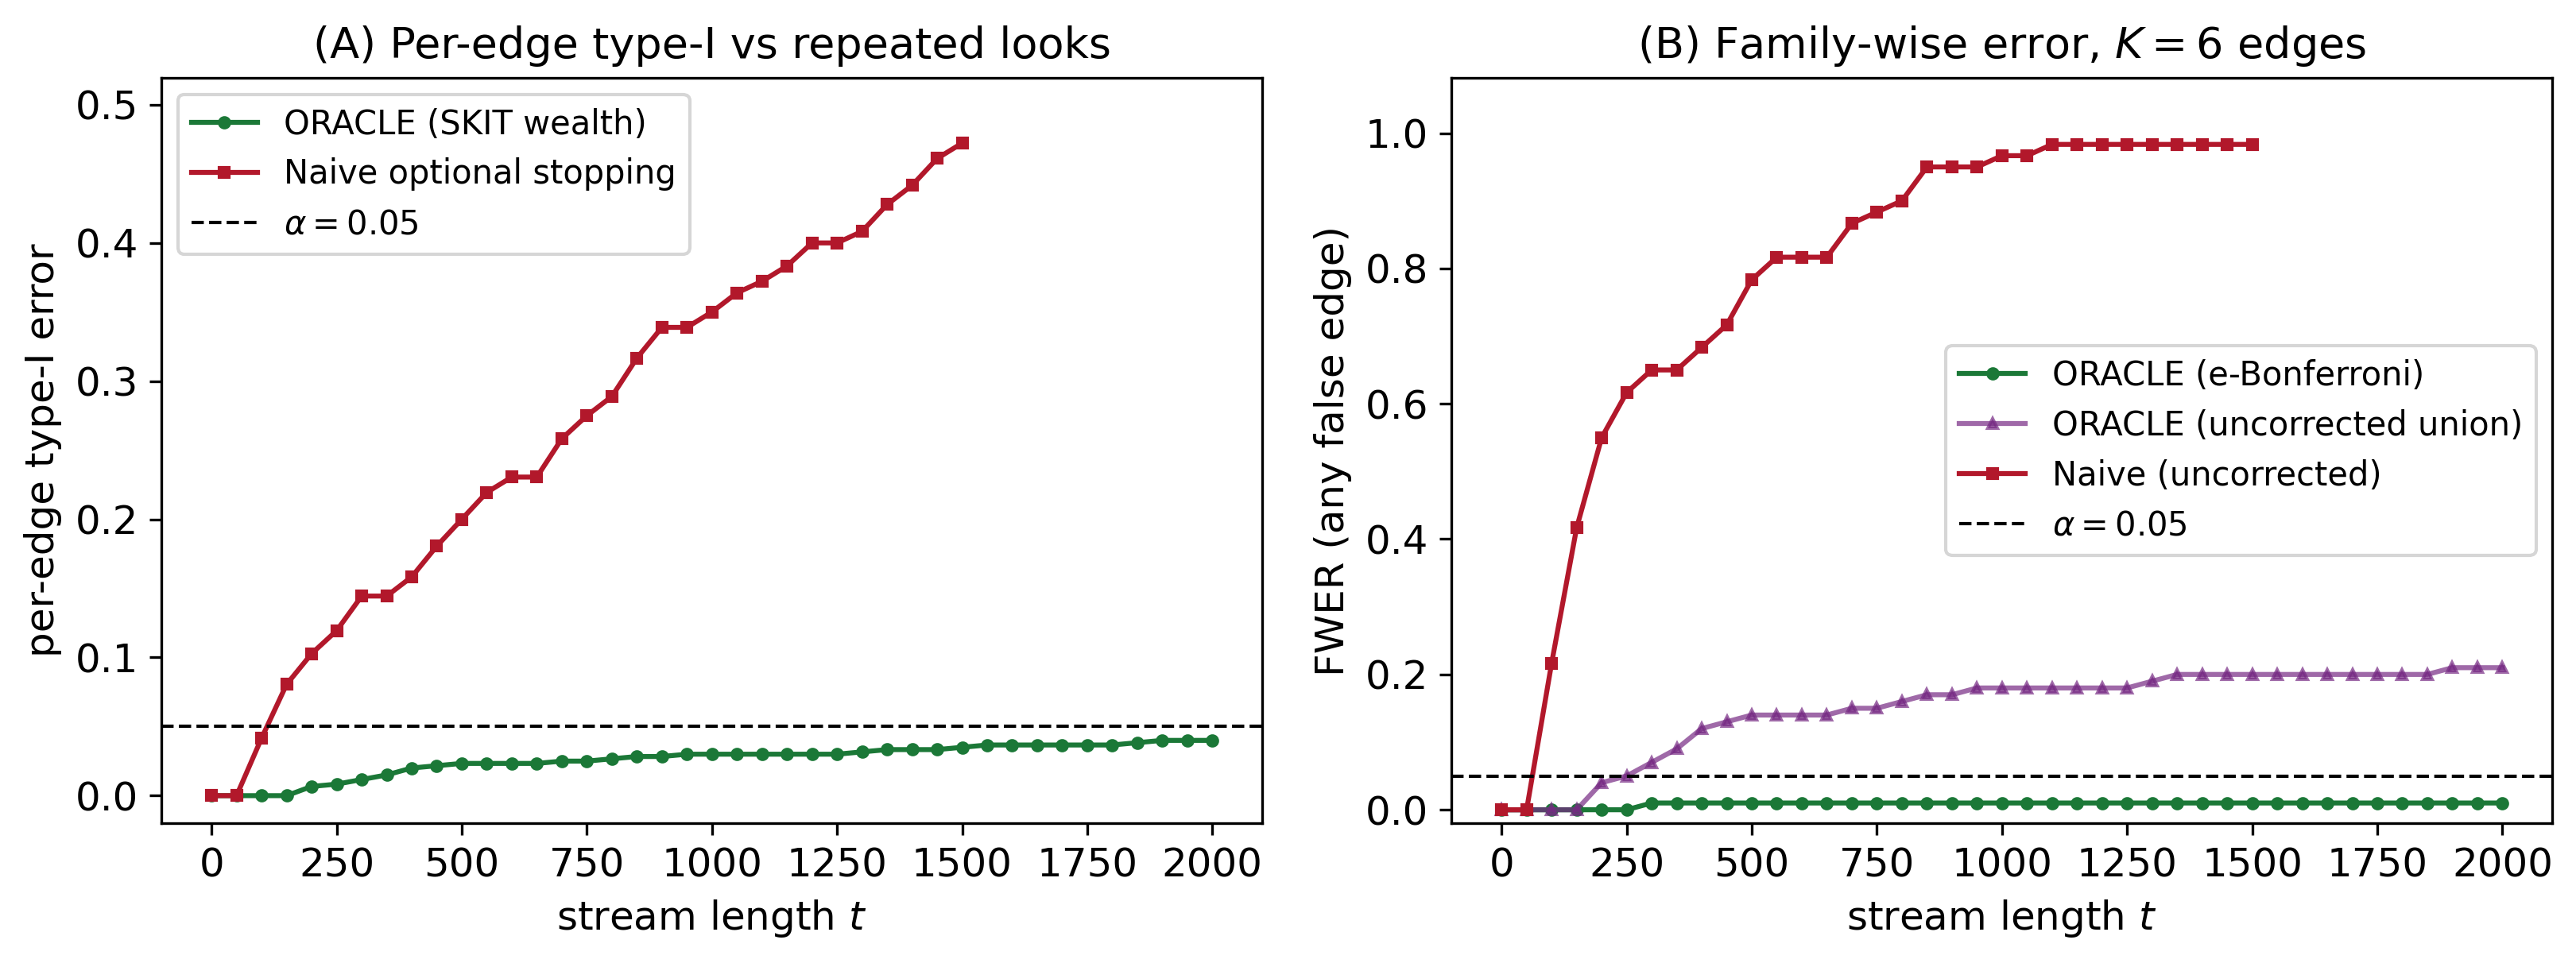
\includegraphics[width=\textwidth]{figures/validity_fwer.png}
    \caption{Validity audit on a null (independent) stream. (A) Per-edge type-I
    error versus stream length: the ORACLE SKIT wealth stays at/below $\alpha$
    for all $t$, the naive optional-stopping $p$-value test climbs. (B)
    Family-wise error across all $K=p(p-1)/2$ candidate edges: ORACLE with e-BH/
    e-Bonferroni remains controlled while the naive union approaches one.}
    \label{fig:validity}
\end{figure}

\begin{table}[htbp]
\centering
\caption{Validity audit on a null stream ($p=4$, $K=6$ edges, target $\alpha=0.05$). ORACLE controls error uniformly over the stream; naive optional stopping inflates. ORACLE column uses e-Bonferroni for FWER.}
\label{tab:validity}
\begin{tabular}{lcc}
\hline
metric & ORACLE (SKIT) & Naive opt.\ stopping \\
\hline
max per-edge type-I & \textbf{0.040} & 0.472 \\
max FWER (any false edge) & \textbf{0.010} & 0.983 \\
\hline
\end{tabular}
\end{table}


\paragraph{Graph recovery.}
On normalised non-Gaussian ANM data, ORACLE's online estimate converges toward
the ground-truth graph as the stream lengthens
(Figure~\ref{fig:recovery_convergence}; Table~\ref{tab:recovery}). On the
Erd\H{o}s--R\'enyi/Laplace settings it attains a structural Hamming and
intervention distance comparable to batch PC-stable and GES---run with full data
access at each checkpoint (Figure~\ref{fig:recovery_comparison})---while
additionally providing the anytime guarantees those batch methods lack. ORACLE
is the more conservative estimator: it tends to declare fewer edges, so its
skeleton recall (and hence skeleton F1) is somewhat lower than the batch
constraint test even when its SHD is on par or better. We also report an honest
failure mode: on the dense scale-free graph with heavy-tailed Student-$t_3$
noise, the online residual regression and kernel-scale estimates degrade and
recovery is poor; this regime stresses the additive-noise and bounded-moment
assumptions the method relies on. The central point is that ORACLE delivers
\emph{competitive} structure recovery \emph{online}, at streaming throughput,
while its distinguishing property---error control at every stopping time
(Section~\ref{sec:results}, validity audit)---is one no batch baseline provides.

\begin{figure}[htpb]
    \centering
    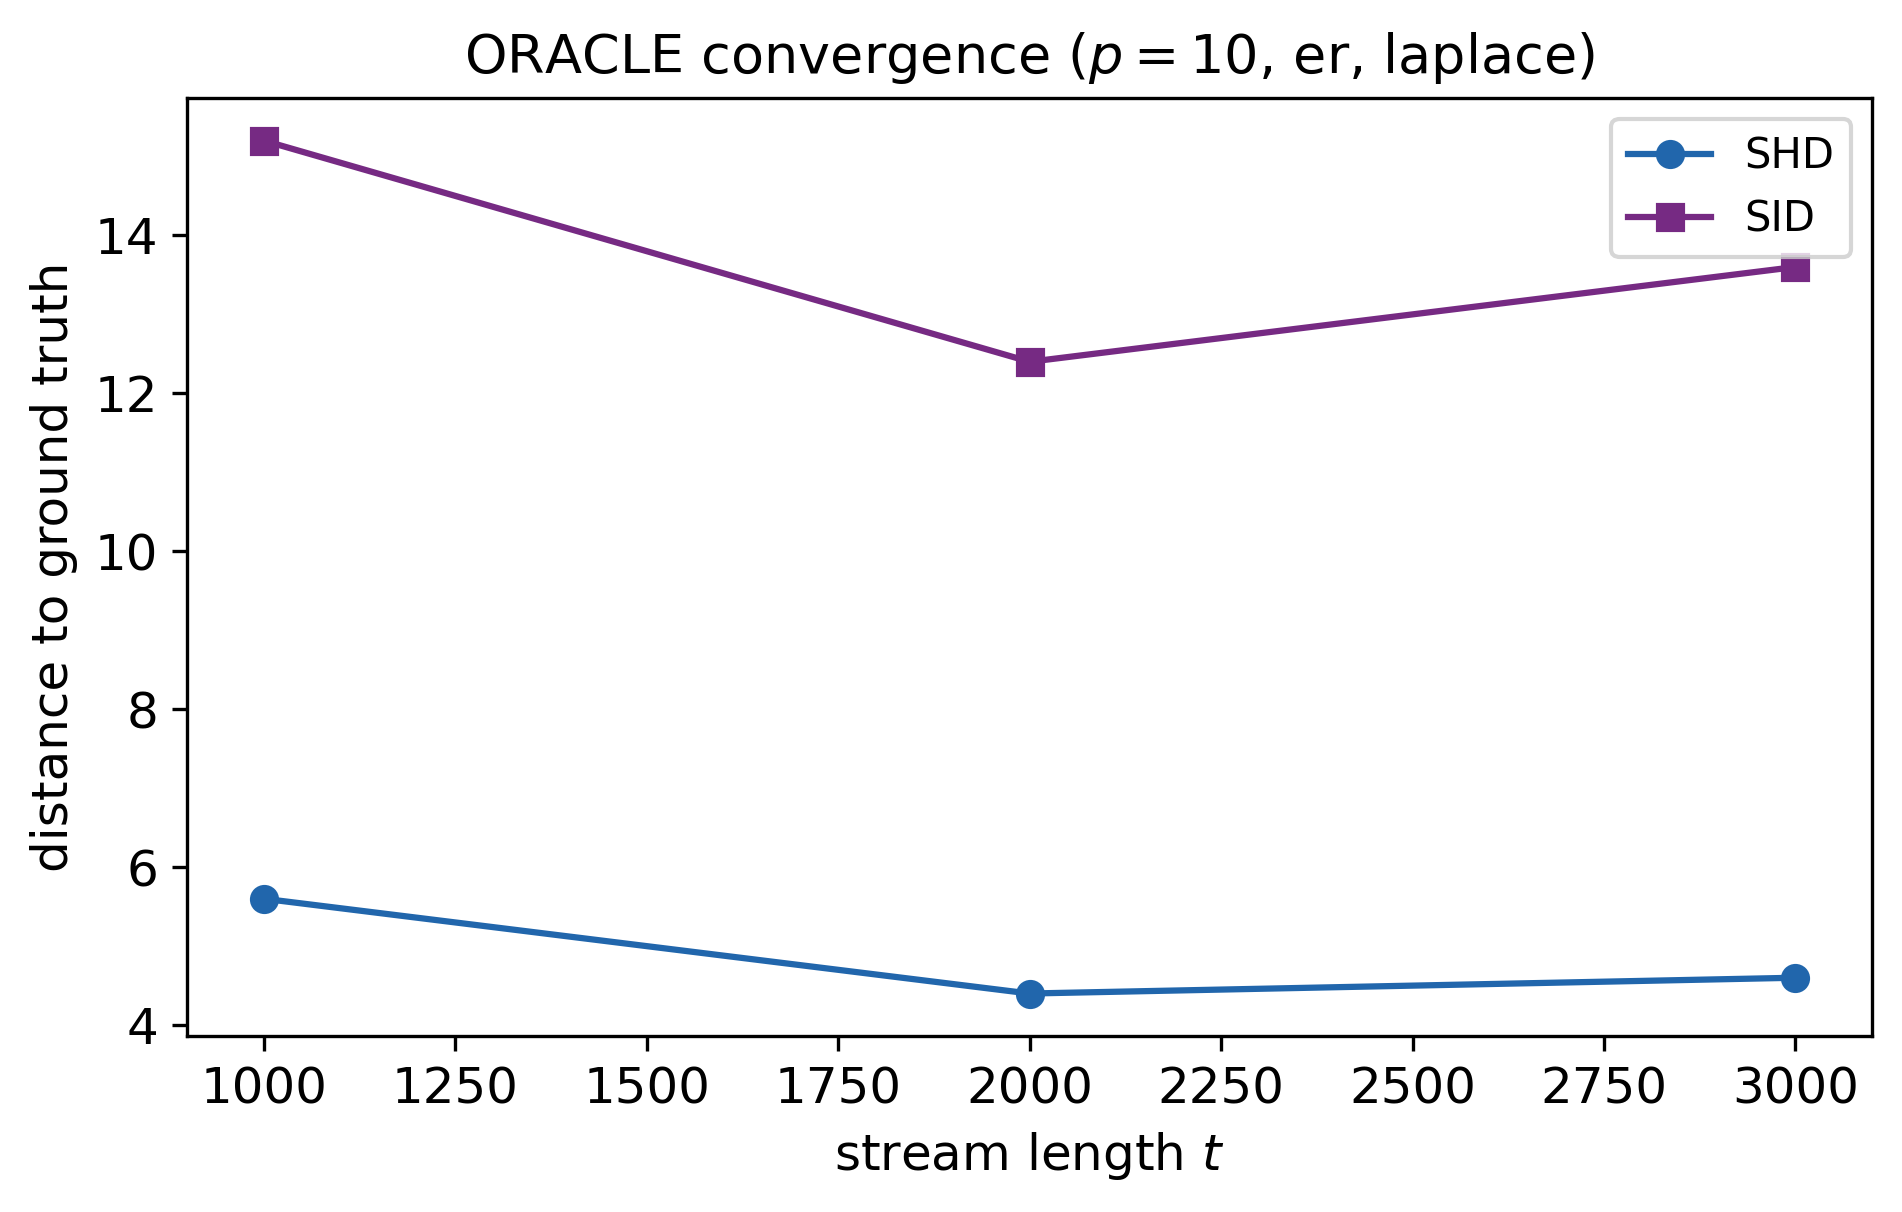
\includegraphics[width=0.7\textwidth]{figures/recovery_convergence.png}
    \caption{ORACLE convergence: structural Hamming and intervention distance to
    the ground-truth DAG as a function of stream length.}
    \label{fig:recovery_convergence}
\end{figure}

\begin{figure}[htpb]
    \centering
    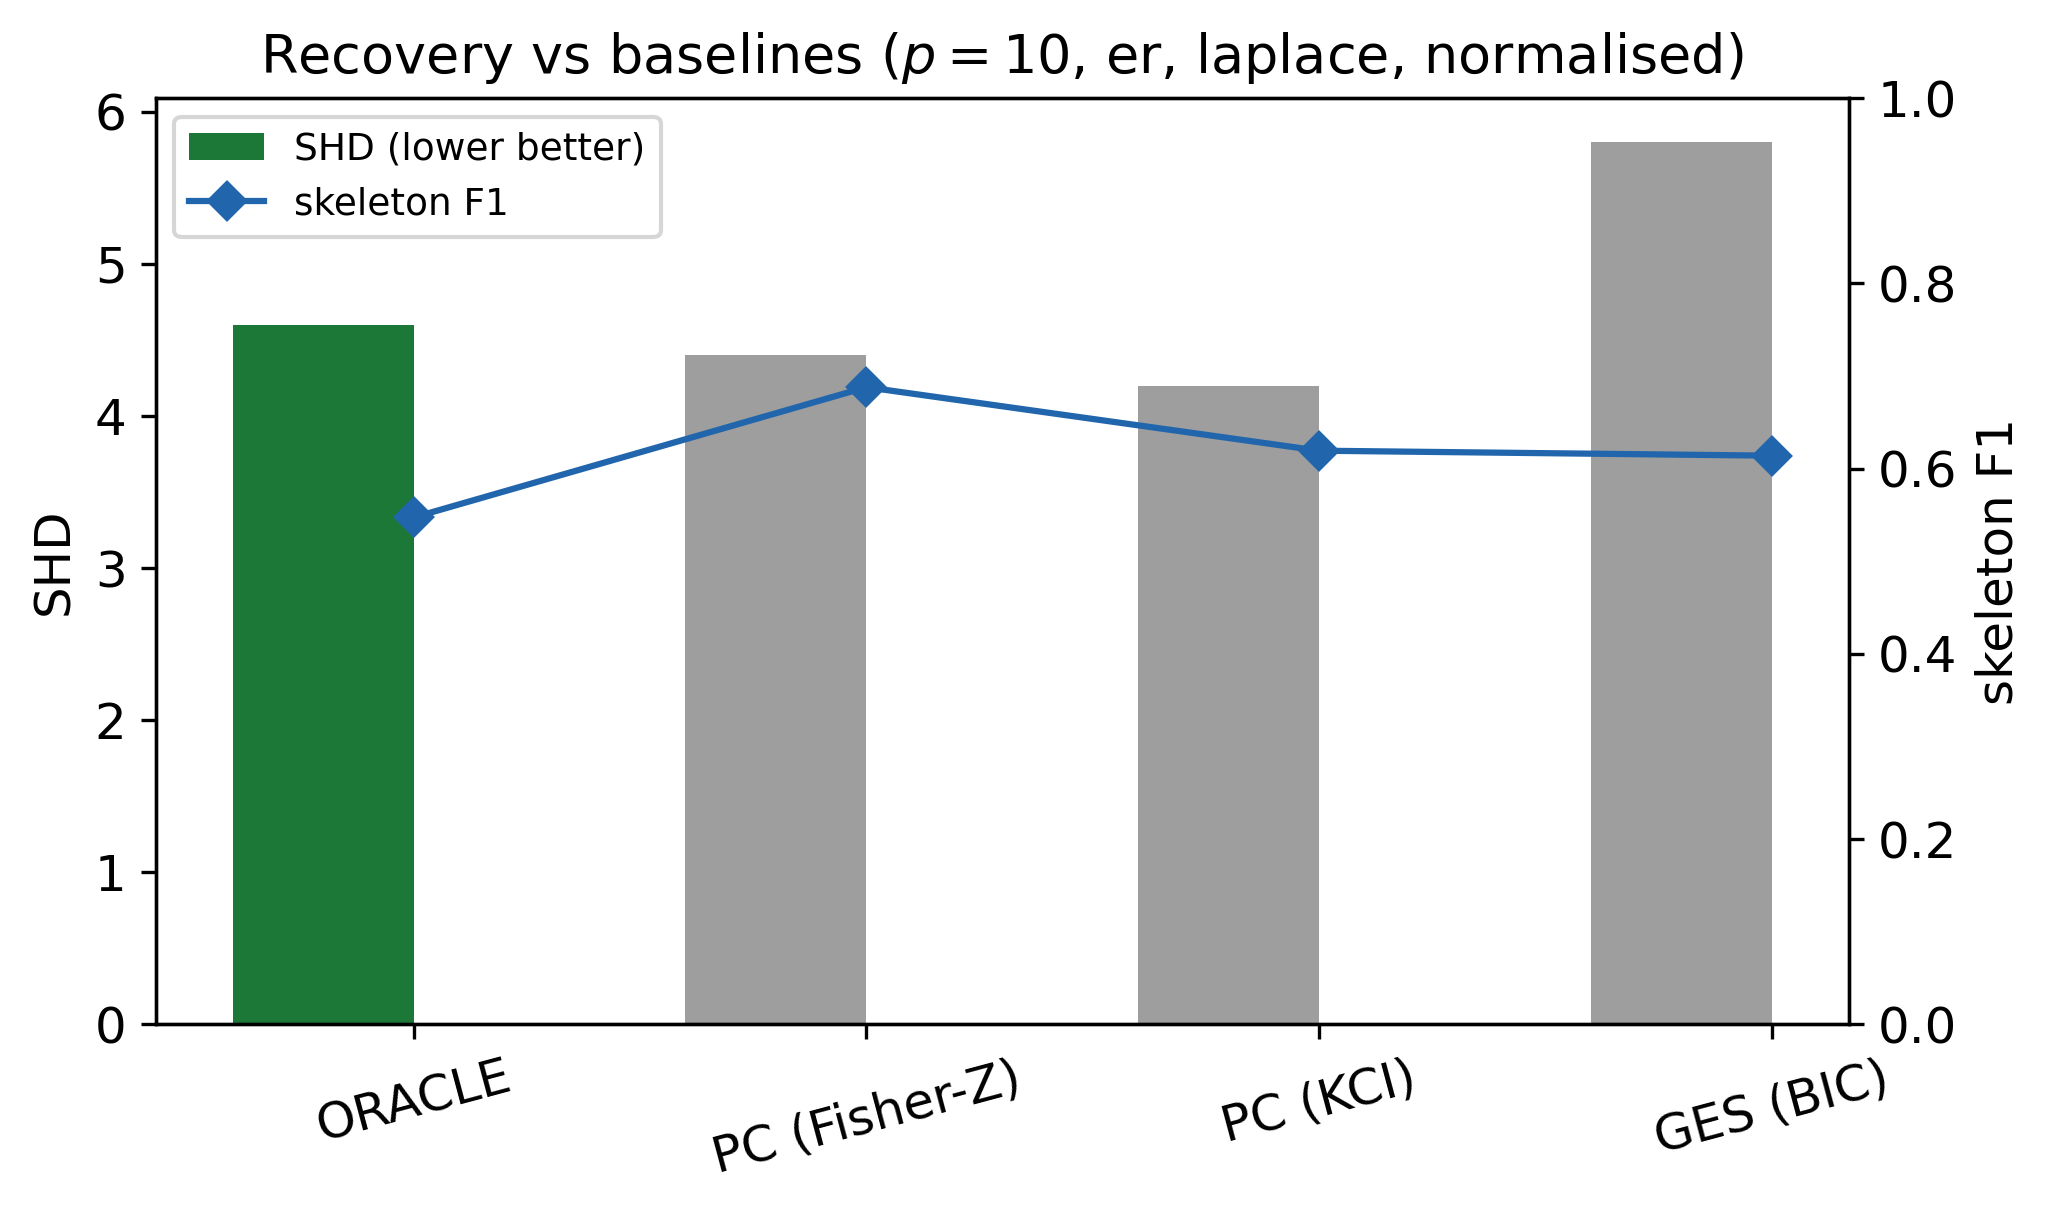
\includegraphics[width=0.75\textwidth]{figures/recovery_comparison.png}
    \caption{Graph recovery versus batch baselines (PC-stable with Fisher-Z and
    KCI, GES) in the checkpoint harness, on normalised data. Bars: SHD (lower is
    better); markers: skeleton F1.}
    \label{fig:recovery_comparison}
\end{figure}

\begin{table}[htbp]
\centering
\caption{Graph recovery on normalised non-Gaussian ANM data: ORACLE (online) versus batch baselines (checkpoint harness). SHD/SID lower is better; F1 higher is better.}
\label{tab:recovery}
\begin{tabular}{lcccc}
\hline
method & SHD & SID & skel.\ F1 & orient.\ F1 \\
\hline
\hline
\multicolumn{5}{l}{\emph{$p=10$, er, laplace noise, density 1.5, $n=3000$ }} \\
\hline
\quad ORACLE & \textbf{4.6} & 13.6 & 0.55 & 0.55 \\
\quad PC (Fisher-Z) & 4.4 & 13.6 & 0.69 & 0.59 \\
\quad PC (KCI) & 4.2 & 9.8 & 0.62 & 0.52 \\
\quad GES (BIC) & 5.8 & 14.6 & 0.61 & 0.54 \\
\hline
\multicolumn{5}{l}{\emph{$p=10$, sf, t3 noise, density 2.0, $n=2500$ }} \\
\hline
\quad ORACLE & \textbf{15.2} & 80.0 & 0.08 & 0.08 \\
\quad PC (Fisher-Z) & 19.5 & 66.0 & 0.57 & 0.29 \\
\quad PC (KCI) & 13.2 & 75.5 & 0.59 & 0.22 \\
\quad GES (BIC) & 23.2 & 55.5 & 0.51 & 0.33 \\
\hline
\multicolumn{5}{l}{\emph{$p=15$, er, laplace noise, density 1.5, $n=2000$ }} \\
\hline
\quad ORACLE & \textbf{10.5} & 29.0 & 0.47 & 0.47 \\
\quad PC (Fisher-Z) & 12.5 & 56.0 & 0.67 & 0.47 \\
\quad PC (KCI) & 10.0 & 62.0 & 0.76 & 0.40 \\
\quad GES (BIC) & 10.5 & 39.0 & 0.74 & 0.57 \\
\hline
\end{tabular}
\end{table}


\paragraph{Anytime behaviour.}
Figure~\ref{fig:anytime} contrasts the accumulation of false skeleton edges over
the stream. ORACLE detects true edges early---at a small fraction of the stream
length---while holding the number of falsely declared edges low and stable. The
naive procedure accrues false edges as the stream grows, the structural
manifestation of the optional-stopping inflation in Figure~\ref{fig:validity}.

\begin{figure}[htpb]
    \centering
    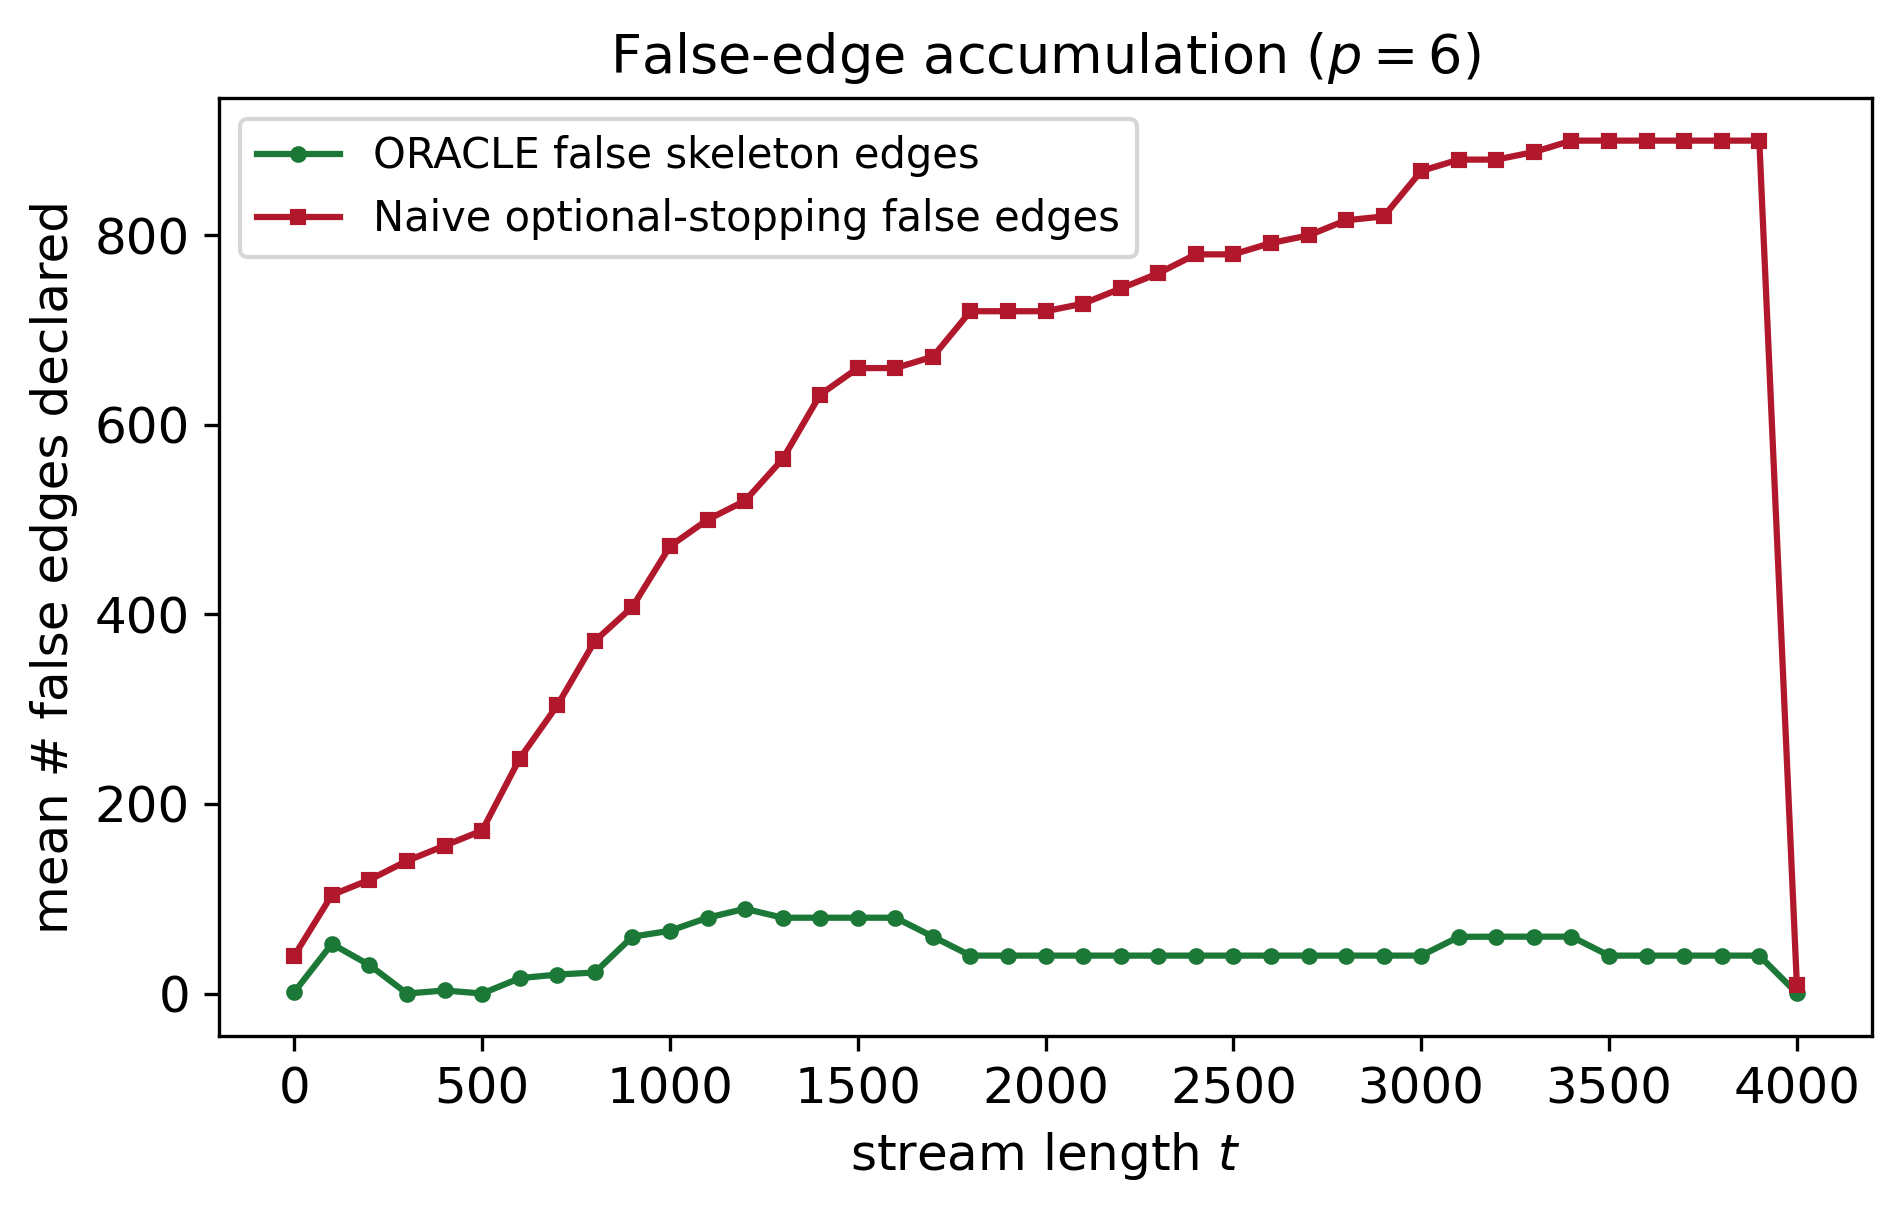
\includegraphics[width=0.7\textwidth]{figures/anytime_false_edges.png}
    \caption{False-edge accumulation over the stream on planted DAGs: ORACLE
    holds false edges low while the naive optional-stopping baseline accumulates
    them.}
    \label{fig:anytime}
\end{figure}

\paragraph{Change detection.}
Sweeping the Page--CUSUM threshold $h$ traces a clean, monotone trade-off between
detection delay and ARL to false alarm (Figure~\ref{fig:change}): larger $h$
lengthens the delay but extends the ARL, and at a moderate threshold the detector
attains full detection of planted mechanism changes with no false alarms before
the change. This gives the analyst a single, interpretable knob to set the
operating point.

\begin{figure}[htpb]
    \centering
    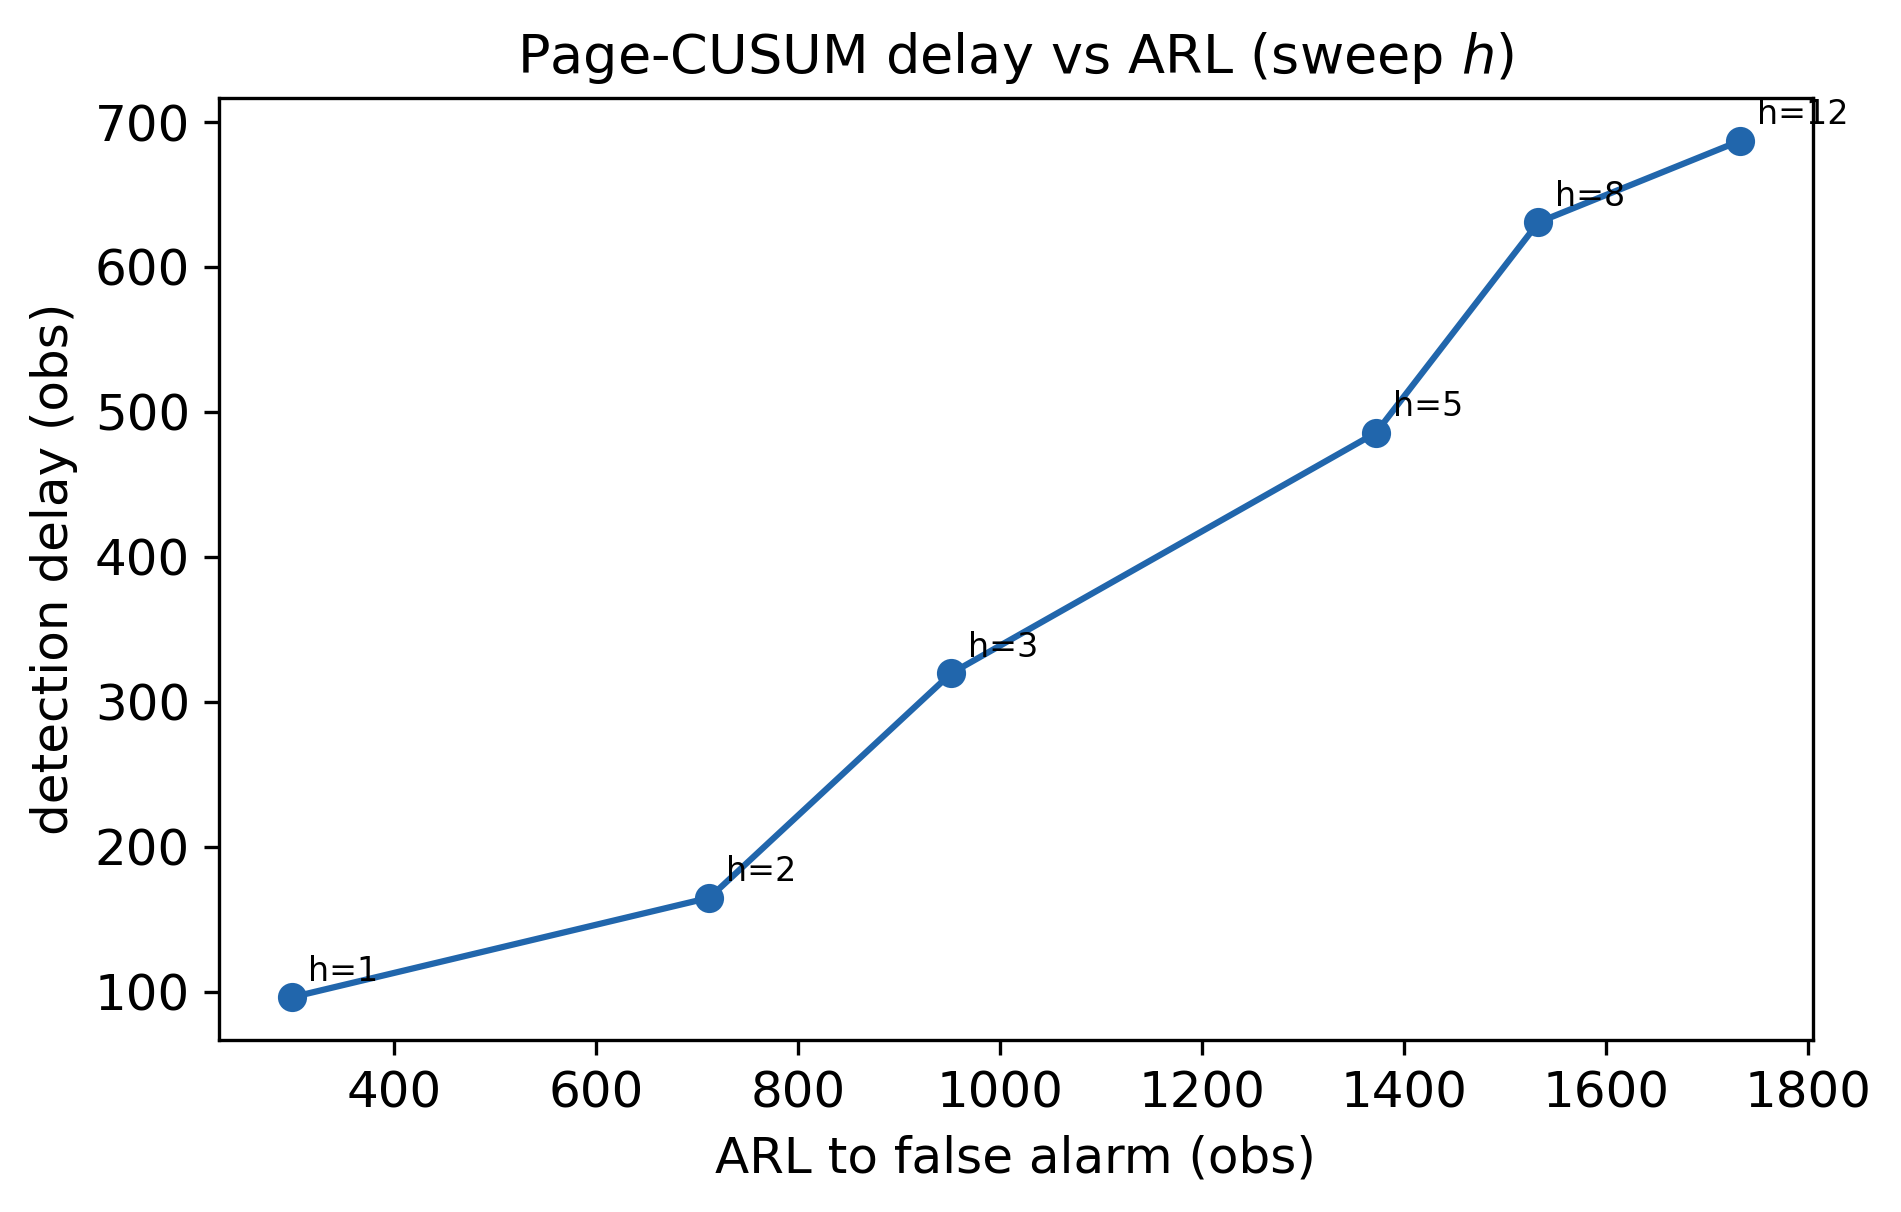
\includegraphics[width=0.7\textwidth]{figures/change_delay_arl.png}
    \caption{Page--CUSUM detection delay versus ARL to false alarm as the
    threshold $h$ is swept on piecewise-stationary streams.}
    \label{fig:change}
\end{figure}

\begin{table}[htbp]
\centering
\caption{Change detection ($p=5$, segment $=1800$, 2 change-points, 16 monitored edges). Page--CUSUM threshold $h$ trades delay against ARL to false alarm.}
\label{tab:change}
\begin{tabular}{cccc}
\hline
$h$ & mean delay & mean ARL & det.\ rate \\
\hline
0.5 & -- & 150 & 0.00 \\
1 & 96 & 299 & 0.06 \\
2 & 165 & 712 & 0.25 \\
3 & 320 & 951 & 0.38 \\
5 & 486 & 1372 & 0.69 \\
8 & 631 & 1533 & 0.75 \\
12 & 687 & 1732 & 0.94 \\
\hline
\end{tabular}
\end{table}


\paragraph{Systems.}
Figure~\ref{fig:systems} reports throughput and peak memory as $p$ grows.
Throughput is in the hundreds of observations per second for small $p$ and
degrades gracefully with the quadratic number of candidate pairs, confirming the
method is usable in real time for moderate-dimensional streams; memory grows
modestly with the RFF and windowed statistics.

\begin{figure}[htpb]
    \centering
    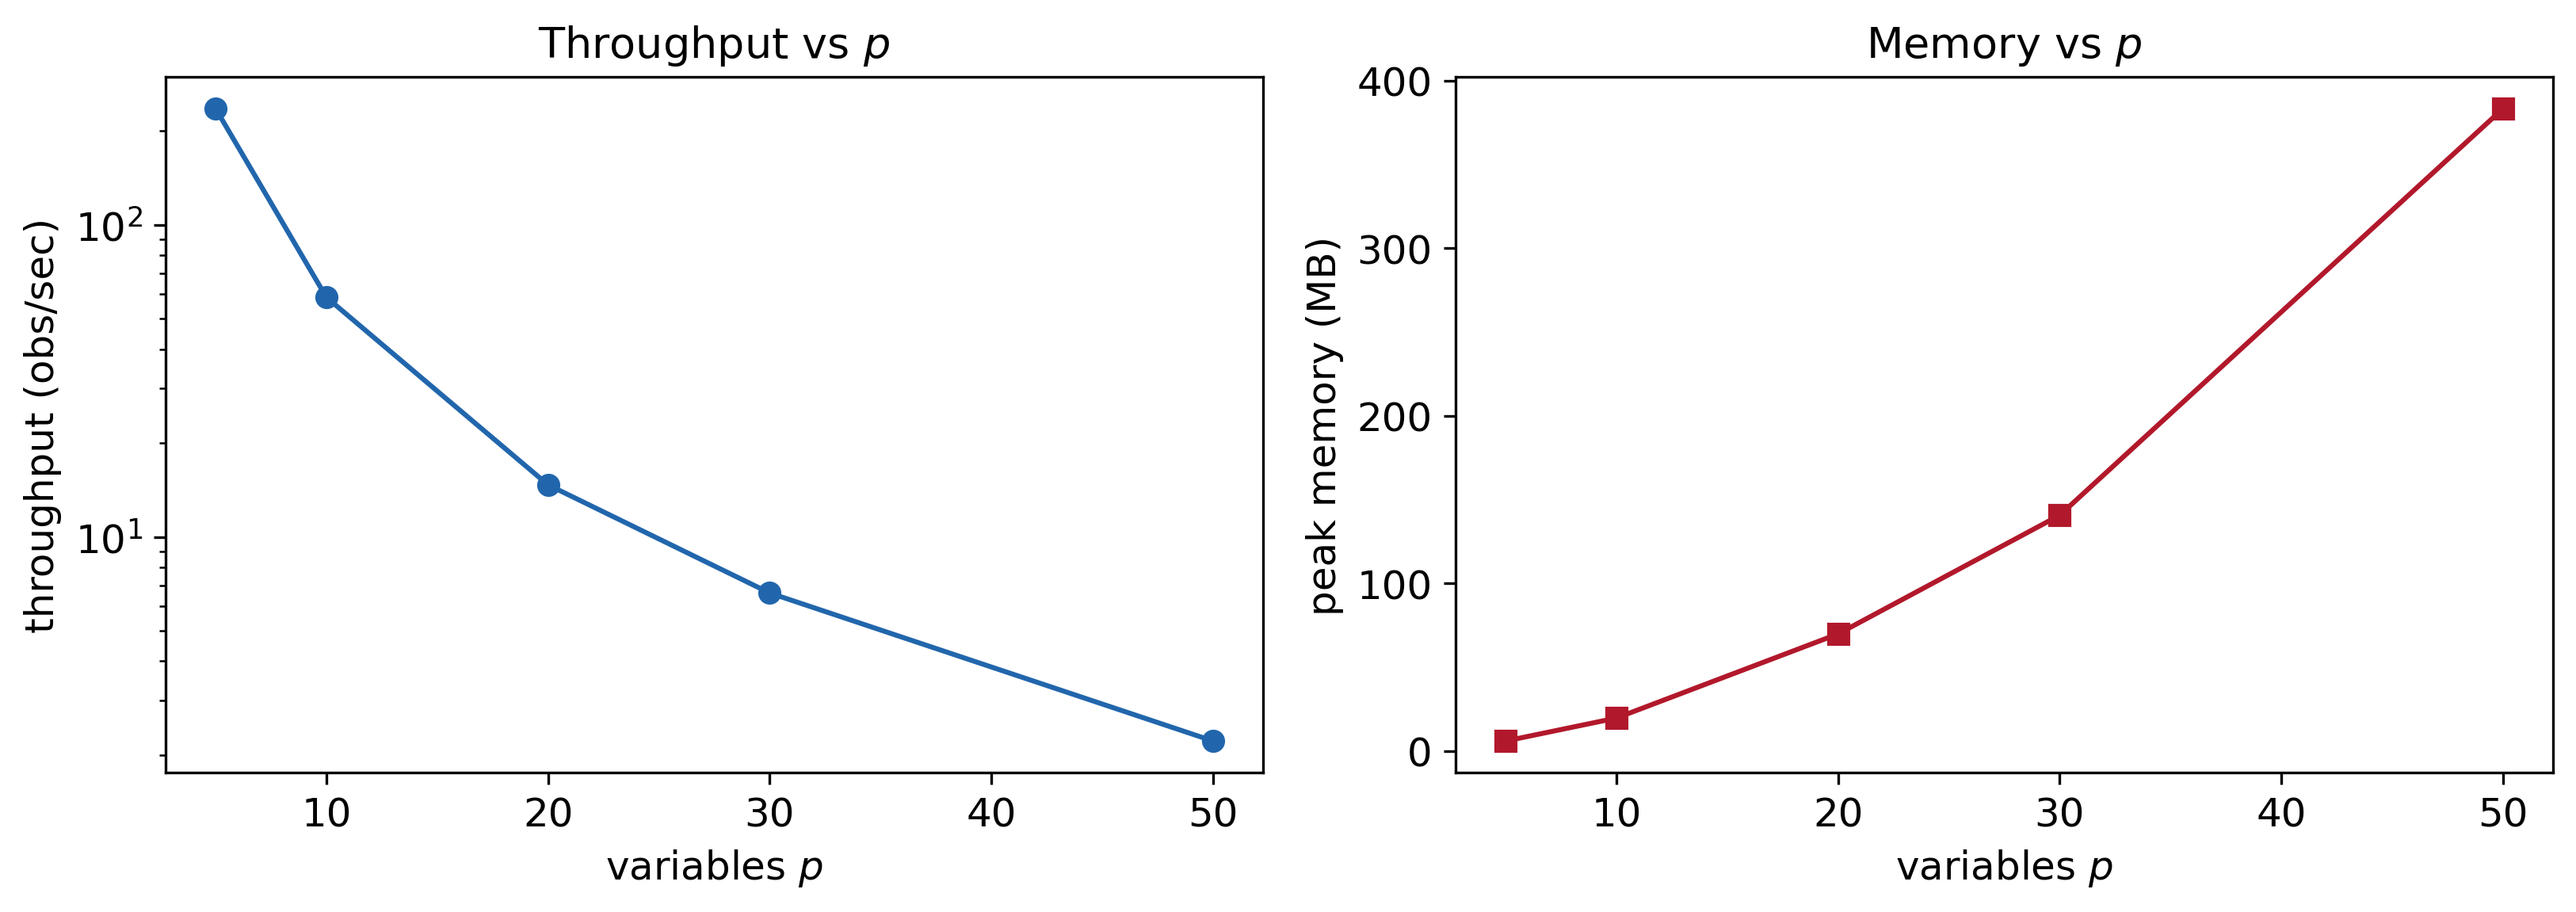
\includegraphics[width=\textwidth]{figures/systems_scaling.png}
    \caption{Throughput (observations/second, log scale) and peak memory versus
    the number of variables $p$.}
    \label{fig:systems}
\end{figure}

\begin{table}[htbp]
\centering
\caption{Systems scaling (stream length $n=800$): throughput and peak memory versus the number of variables $p$.}
\label{tab:systems}
\begin{tabular}{ccccc}
\hline
$p$ & pairs & RFF $D$ & obs/sec & mem (MB) \\
\hline
5 & 10 & 64 & 236 & 5.8 \\
10 & 45 & 64 & 59 & 19.5 \\
20 & 190 & 64 & 15 & 69.8 \\
30 & 435 & 32 & 7 & 140.6 \\
50 & 1225 & 32 & 2 & 383.4 \\
\hline
\end{tabular}
\end{table}


\paragraph{Ablations.}
We ablate every major design choice on a fixed family of synthetic ANM DAGs;
exact numbers are reported in the tables, and we summarise the trends here.
The \emph{degree cap} $k$ (Table~\ref{tab:abl_k}, Figure~\ref{fig:ablation})
controls a cost/correctness trade-off rather than a uniform improvement: on the
sparse random graphs of this benchmark the unconditioned pairwise skeleton
($k=0$) is already accurate and increasing $k$ can reduce recall through
over-conditioning by the online regressors, whereas conditioning is
\emph{provably} required to remove edges between variables that are dependent
marginally but independent given a separating set---the chain
$X\to Y\to Z$ with $X\perp\!\!\!\perp Z\mid Y$ of our consistency test
(Section~\ref{sec:ci}), where $k=0$ cannot recover the DAG. The cap should
therefore be set to the largest in-degree one expects, not larger. The
\emph{significance level} $\alpha$ (Table~\ref{tab:abl_alpha}) trades precision
for recall. \emph{Bet sizing} (Table~\ref{tab:abl_bet}) compares fixed, aGRAPA,
and the parameter-free mixture; all three are anytime-valid by construction and
differ only in power, with the ranking inside the noise of this small-graph
regime. The \emph{RFF feature count} $D$ (Table~\ref{tab:abl_features}) shows
recovery is not sensitive to $D$ over the tested range. \emph{Multiplicity
control} (Table~\ref{tab:abl_mult}) contrasts e-BH, e-Bonferroni, and no
correction. The \emph{noise family} (Table~\ref{tab:abl_noise}) probes
robustness across Laplace, Student-$t_3$, and Gumbel noise, with Gaussian noise
included as the non-identifiable control where the additive-noise direction is
provably unrecoverable. The \emph{warm-up window} (Table~\ref{tab:abl_warmup})
varies the previsibility initialisation length. Finally, the
witness-standardisation study (Table~\ref{tab:abl_std}) isolates the single
change that makes the betting test powerful: without standardisation the small
HSIC signal yields negligible wealth growth and the test rarely rejects, whereas
standardising by the previsible running scale recovers high power without
affecting validity.

\begin{figure}[htpb]
    \centering
    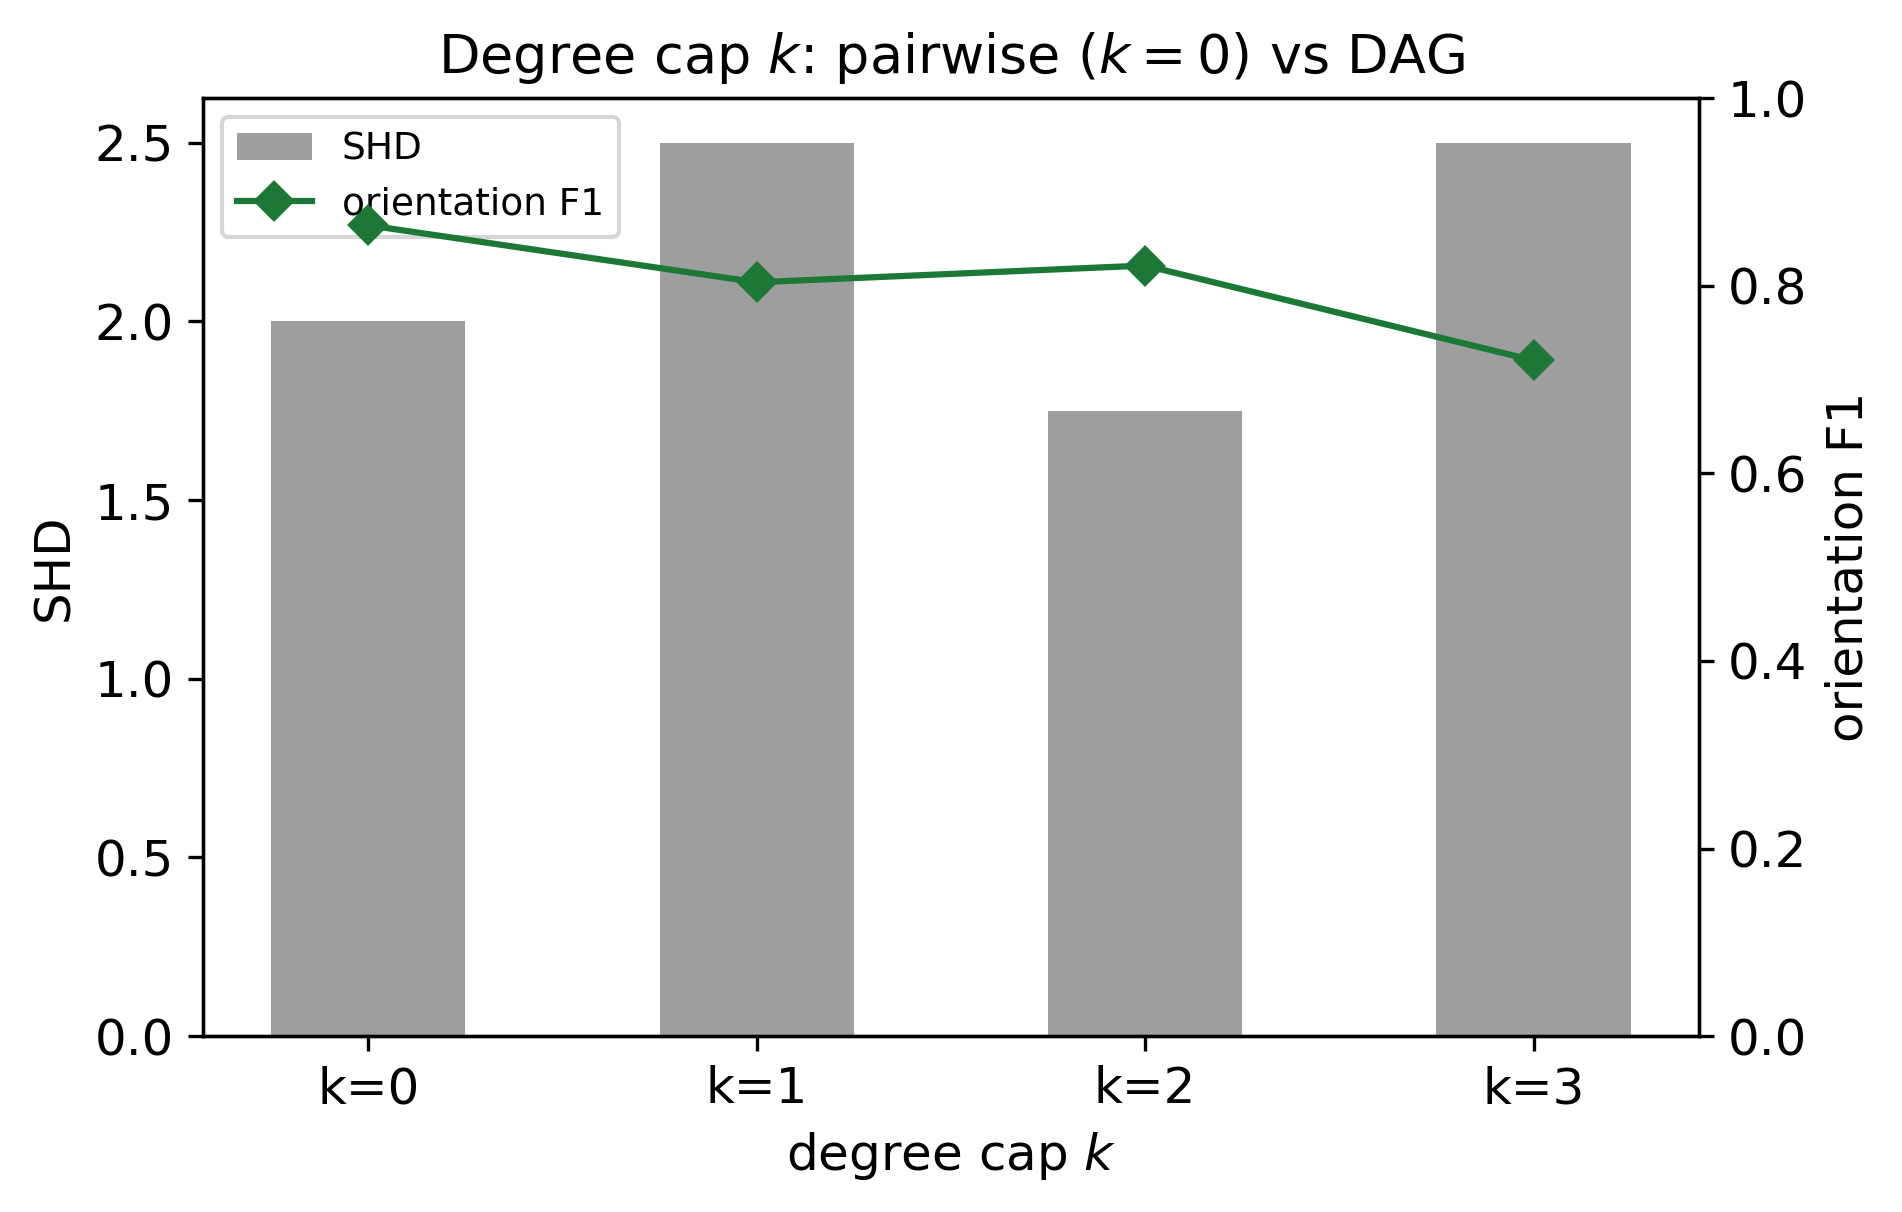
\includegraphics[width=0.7\textwidth]{figures/ablation_degree_cap.png}
    \caption{Degree-cap ablation. Bars: SHD; markers: orientation F1. On these
    sparse random graphs the unconditioned skeleton ($k=0$) is already accurate;
    the cap trades cost against the ability to remove edges explained away by a
    separating set (required on chains/colliders, cf.\ Section~\ref{sec:ci}).}
    \label{fig:ablation}
\end{figure}

\begin{table}[htbp]
\centering
\caption{Ablation: degree cap $k$ ($k=0$ is a pairwise dependency graph, not a DAG).}
\label{tab:abl_k}
\begin{tabular}{lcccc}
\hline
$k$ & SHD & SID & skel.\ F1 & orient.\ F1 \\
\hline
0 & 2.0 & 3.2 & 0.89 & 0.86 \\
1 & 2.5 & 3.8 & 0.80 & 0.80 \\
2 & 1.8 & 5.2 & 0.89 & 0.82 \\
3 & 2.5 & 7.5 & 0.80 & 0.72 \\
\hline
\end{tabular}
\end{table}

\begin{table}[htbp]
\centering
\caption{Ablation: significance level $\alpha$.}
\label{tab:abl_alpha}
\begin{tabular}{lcccc}
\hline
$\alpha$ & SHD & SID & skel.\ F1 & orient.\ F1 \\
\hline
0.01 & 1.0 & 3.0 & 0.91 & 0.91 \\
0.05 & 2.2 & 5.2 & 0.77 & 0.77 \\
0.1 & 2.2 & 6.5 & 0.80 & 0.75 \\
\hline
\end{tabular}
\end{table}

\begin{table}[htbp]
\centering
\caption{Ablation: bet sizing.}
\label{tab:abl_bet}
\begin{tabular}{lcccc}
\hline
bet & SHD & SID & skel.\ F1 & orient.\ F1 \\
\hline
fixed & 2.5 & 5.2 & 0.75 & 0.75 \\
agrapa & 2.8 & 5.8 & 0.72 & 0.72 \\
mixture & 3.2 & 8.0 & 0.63 & 0.63 \\
\hline
\end{tabular}
\end{table}

\begin{table}[htbp]
\centering
\caption{Ablation: RFF feature count $D$.}
\label{tab:abl_features}
\begin{tabular}{lcccc}
\hline
$D$ & SHD & SID & skel.\ F1 & orient.\ F1 \\
\hline
32 & 3.0 & 6.8 & 0.67 & 0.59 \\
64 & 3.0 & 7.2 & 0.67 & 0.59 \\
128 & 3.2 & 6.8 & 0.64 & 0.56 \\
\hline
\end{tabular}
\end{table}

\begin{table}[htbp]
\centering
\caption{Ablation: multiplicity control.}
\label{tab:abl_mult}
\begin{tabular}{lcccc}
\hline
method & SHD & SID & skel.\ F1 & orient.\ F1 \\
\hline
ebh & 1.0 & 2.0 & 0.90 & 0.90 \\
bonferroni & 1.2 & 2.5 & 0.86 & 0.86 \\
none & 1.0 & 2.0 & 0.90 & 0.90 \\
\hline
\end{tabular}
\end{table}

\begin{table}[htbp]
\centering
\caption{Ablation: noise family (Gaussian is the non-identifiable control).}
\label{tab:abl_noise}
\begin{tabular}{lcccc}
\hline
noise & SHD & SID & skel.\ F1 & orient.\ F1 \\
\hline
laplace & 2.2 & 4.0 & 0.68 & 0.68 \\
t3 & 1.8 & 3.0 & 0.78 & 0.78 \\
gumbel & 1.5 & 2.5 & 0.81 & 0.81 \\
gaussian & 4.0 & 8.0 & 0.30 & 0.30 \\
\hline
\end{tabular}
\end{table}

\begin{table}[htbp]
\centering
\caption{Ablation: warm-up window length.}
\label{tab:abl_warmup}
\begin{tabular}{lcccc}
\hline
warm-up & SHD & SID & skel.\ F1 & orient.\ F1 \\
\hline
25 & 2.8 & 8.0 & 0.69 & 0.62 \\
40 & 2.5 & 7.5 & 0.72 & 0.64 \\
60 & 2.8 & 8.0 & 0.69 & 0.62 \\
\hline
\end{tabular}
\end{table}

\begin{table}[htbp]
\centering
\caption{Ablation: witness standardisation (SKIT-level power study on a fixed dependent stream). Standardisation turns the small HSIC signal into an order-one payoff.}
\label{tab:abl_std}
\begin{tabular}{lcc}
\hline
standardisation & rejection rate & median detection \\
\hline
on & 1.00 & 84 \\
off & 1.00 & 399 \\
\hline
\end{tabular}
\end{table}


%% ===================================================================
\section{Discussion and Conclusion}
\label{sec:conclusion}
We have presented ORACLE, an online causal-discovery procedure that controls the
false-edge rate at every stopping time by replacing the conditional-independence
$p$-value with a sequential test by betting. The empirical study confirms the
central claim: under optional stopping ORACLE holds error at the nominal level
uniformly over the stream while a naive repeated-looks baseline inflates toward
certainty, and it does so without sacrificing competitive structure recovery,
a controllable change-detection trade-off, or streaming throughput.

Several limitations point to future work. Orientation uses the bivariate
additive-noise asymmetry; with multiple parents and strong nonlinearity the
pairwise residual may be imperfect, and a fully parent-conditioned orientation
test would strengthen identifiability. The guarantees rest on each increment
being a valid e-value under additive structure; when this is violated ORACLE
surfaces the conflict by leaving edges undirected rather than committing, which
is honest but reduces orientation recall. Scaling to large $p$ is bounded by the
quadratic number of candidate pairs; sketching or Markov-blanket-restricted
candidate generation would extend the reach. Finally, the same betting machinery
applies directly to interventional and time-lagged settings, which we leave for
future study.

\section*{Code and Data Availability}
A complete reference implementation of ORACLE, together with the synthetic data
generators, the full evaluation suite, and scripts that reproduce every figure
and table in this paper, is openly available at
\url{https://github.com/vinhqdang/anytime-causal}. All experiments use synthetic
data generated by the released code from fixed random seeds; because the method
is a streaming, stochastic procedure, re-runs may differ negligibly from the
reported values, and the repository regenerates results, figures, and tables
end-to-end.

\section*{Acknowledgements}
The author would like to thank colleagues at British University Vietnam for
helpful discussions.

%% Bibliography
\bibliographystyle{elsarticle-harv}
\bibliography{references}

\end{document}
